\documentclass[11pt]{article}
\usepackage{amsmath}
\usepackage{amsfonts}
\usepackage{ntheorem}
\usepackage[margin=1in]{geometry}
\usepackage{graphicx}
\usepackage{amssymb}
\usepackage{algorithm,algorithmicx}
\usepackage[noend]{algpseudocode}
\newtheorem{definition}{Definition}
\newtheorem{function}{Function}
\graphicspath{{./PNgraph/}}

\begin{document}
\title{Implement Unfolding based POR Algorithm}
\author{Huyen Nguyen}
\date{\today}
\maketitle

\section{Building labelled event structure - parametric semantics}
\subsection{Define the independent relation}

\begin{definition}{Commutativity}
	Two transitions t and t' are commuted if at every state (reachable marking) s:
	\begin{enumerate}
		\item $t, t'\in enable(s) and s\rightarrow ^t s' \Longrightarrow t'\in enable(s')$ 		
		
		$ fire(s,t)$ is a new state reached by firing t at s
		\item $t, t' \in enable(s) and \exists s": s\xrightarrow{t.t'} s" then s\xrightarrow{t'.t} s"$ 
		
	\end{enumerate}
\end{definition}

	Set up independent set:
	\begin{itemize}
	\item compute all reachable markings (already implemented in simple model checker SMC)
	\item For all pairs $(t_1,t_2)$, check if $t_1$ and $t_2$ commute or not: $check\_commute(t_1,t_2)$ 
	\item if yes, store all independent pairs in a set
	\end{itemize}	
	
\begin{algorithm}{}
\caption{Commutativity algorithm}\label{alg:cmt}
\begin{algorithmic}[1]
\Function {$check\_commute$}{$a,b$}
 	\For {reachable markings s}
		\If {s enables one of t and t'}
			\State{return false}
		\Else
			\If{s enables both t and t'}
				\State {s'= fire(s,t)}
				\State {s"= fire(s,t')}
				\If {s' enables t' and (fire(s',t') == fire(s",t))}
					\State {continue}
				\Else
					\State {return false}
				\EndIf
			\EndIf
		\EndIf
	\EndFor
	\Return{true}
\EndFunction
\end{algorithmic}
\end{algorithm}


\subsection{Construct unfolding under the independent relation for a petri net}
	This part details the process of constructing the unfolding (set of prefix) for a petri net under independent 			relation defined in previous section.
	
	Unfolding is a LES, tuple $\varepsilon$ = $\langle E,<,\#,h\rangle$, where E is a set of events, $<$ is set of 			pairs of events in causal relation, $\#$ is set of events in conflict.
	
	\begin{definition}{Construct the unfolding LES}
	
	\begin{enumerate}
		\item Initially, LES having one event $bottom \perp$
		
		\item Let $\varepsilon$ be an prefix containing a history H (one element in the set of possible histories of 				LES) for some transition t $\in$ T.
		
	\end{enumerate}
	\end{definition}
	
	\begin{verse}
		$\varepsilon$ is a unfolding prefix, initially $\varepsilon=\bot$\\
		\texttt{$//$ check only maximal event because all extendable events had already been computed and added 					to the stack \textbf{extendable} in previous step } 
		$//$ can't find $<e_i.lbl,t>$ in independent set

	\end{verse}


\begin{algorithm}
\caption{Extend LES}
\begin{algorithmic}[1]
\Procedure {Extend}{}
\State {extStack := $\bot$}
	\While {\let\emptyset\varnothing extStack != $\emptyset$}
		\State {Pop up an event e from the stack}
		\State {Marking $s:= state(e_i)$}
		\State {Get all transitions activated (enabled) at s}
	 	\If {$t, e.lbl$ are not independent}
			\State {make a new Event with $lbl=t$; $his =\{e\}$}
			\State {add it to the stack \textbf{extendable}}
		\Else
			\State {search in set of events of LES, if exists an event $e'$ with label t}
			\State {compute the $state(\sigma)$ with a run $\sigma=t.(e.lbl)$ or $(e.lbl).t$}
			\State {find all enabled transitions t' at that state}
			\State {creat new event with $\langle t',\{e,e'\}\rangle$ and compute the reached state}
			\State {Add event to the stack \textbf{extendable}}
		\EndIf
		\State {add e to LES; \textbf{extendable} and add it to LES}
		\State {Compute set of transitions in conflict with e}
	\EndWhile
	\EndProcedure
\end{algorithmic}
\end{algorithm}

	
	To implement the algorithm, we construct a class Event:
	
	\begin{definition}{Event\\}
		class Event\\
		\{ 
		
		Transition lbl; 	$\backslash\backslash$ the transition labels the event
		
		Config his; 	$\backslash\backslash$ histort: set of all predecessors
		
		set$\langle$Event$\rangle$ cfl;$\backslash\backslash$ set of events conflicting with the event
		
		Marking state;
		
		\textup{public:}
		
		void computeCfl();
		
		bool is\_inHis(Event)
		
		bool enable(Transition);
		
		void setState();\\	
		\}
	\end{definition}
		
\begin{definition}{Configuration} \\
	class Config\\
	\{
	
		set $\langle Event \rangle$  event ; maximal events (no more event which is enabled at them) \\
		\textup{member function:}
		
		Marking computeState();
		
		bool is\_inConfig(Event);
	\}
\end{definition}

\begin{definition}{Labelled Event Structure LES}

	set of history of a prefix $<$
	
	The process of buiding the computation tree:
	
	class LES
	
	\{
	
		set $\langle Event \rangle$ evt;
		
		set $\langle Event,Event \rangle$ causal; not necessary
		
		set $\langle Event,Event \rangle$ conflict; not necessary
	
		Marking computeState
		
	\}
\end{definition}


\begin{function}{Compute set of conflict events in LES}	\\ 
	Function computeCfl(e)\\
	\{\\
	  for all event \textbf{e'} in LES.evt
	  
	  	if $(e'.is\_inHis(e)==false)\&\& ((e.is\_inHis(e')==false)) \&\& is\_depend(e.lbl,e'.lbl)$ 
	  	
	  	then
	  	
	  		add e'to e.cfl;
	  		
	  	end if \\
	  \}
\end{function}	

\begin{function}{Check if t and t'independent} \\
	is\_depend(t,t')\\
	\{
	
		for each pair $(t_1,t_2)$ in independent set
		
		if $(t,t')==(t_1,t_2)$
		
		then return true;\\
	\}		
\end{function}

\begin{function}{Check if event e in History of an event}\\
	is\_inHis(e)\\
	\{
	
		$\backslash*$ return true when e is a event in the calling event.$*\backslash $
	
		for each event $e_i$ in his
	
		if $(e == e_i) $ return true;
	
		return false;\\
	\}	
\end{function}

\begin{function}{Check if t enabled at state of some event}\\
	enable(Transition t)\\
	\{

		$\backslash*$ return true when t is activated at the state of that event.$*\backslash $
	
		return state.activates(t); $\backslash*$ activate(t) is a member function in class Marking $*\backslash $ \\
	\}	
\end{function} 
						
\section{LES exploration}

	Given a prefix unfolding in terms of sets of events like picture attached.

	\begin{figure}
		%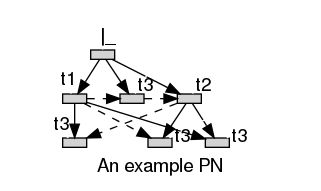
\includegraphics[scale=0.9]{unf.png}
	\end{figure}

	\subsection{Overall algorithm}
	\begin{verse}
			
		U is a virtual set of all events with attribute $seen=true$
	
		G is a virtual set of all events with attribute $in\_gabage=true$
		
		D is a virtual set of all events with attribute $disbale=true$
		
		A is a virtual set of all events with attribute $add=true$
		
		Attribute $visited$ of an event increases by 1 whenever it is visted
		
		C is a configuraition which also store the maximal events. All events in c are marked with $in\_C=true$
		
		J is a configuration possible to add after C as alternative to D
		
	\end{verse}
	
		\begin{algorithm}
		\caption{: POR Exploration algorithm}
		\begin{algorithmic}[1]
			\Procedure {Explore}{C,D,A}
				\State {Extend(C)}
				\let\emptyset\varnothing
				\If {$ en(C) = \emptyset $}
					\Return {}
				\EndIf
				\If {$A=\emptyset$}
					\State {	\textup{Choose e from en(C)}}
				\Else
					\State {e form $A\cap en(C)$}
				\EndIf
				
				\State {Explore($C\cup\{e\},D,A\setminus\{e\}$ )}
				
				\If {$\exists J \in Alt(C,D\cup\{e\})$}
				
					\State {$Explore(C,D\cup\{e\},J\setminus C)$}
				\EndIf
				\State {Remove(e,C,D)}
			\EndProcedure
		\end{algorithmic}
		\end{algorithm}
		
		\begin{algorithm}
		\caption{find alternative event}
		\begin{algorithmic}
			\Procedure {findAlt}{\thickspace}
				\State possible :=true
				\For {each event e in U}
					\If {maximal events of C are in history of e}
						\For {all events e' in D - $disable=true$}
							\If {e not conflict with e'}
								\State {possbile=false}								
								\State {break}
							\EndIf
						\EndFor
						\If {possible==true}
							\State {$J:=J + \{e\}$}
						\EndIf
					\EndIf
				\EndFor		
			\EndProcedure
		\end{algorithmic}
		\end{algorithm}
		
	\subsubsection{A configuration}
		
		\textit{A configuration is a set of events that are causally closed and conflict free.}
		
		- Declared as a set of maximal events
		
		- Member function: 
			
			+ computeState(C) : compute marking reachable by running set of events in C
			
		\subsubsection{Compute ex(C)}
		Compute a set of events extendable at a given configuration C
		\begin{algorithm}
		\begin{algorithmic}
			\Function {ex}{C}
				\For {all events e in LES}
					\If ($e'in e.his$ and $e'.in\_C=true$)
						\State {add e to ex}
					\EndIf
				\EndFor
			\Return {ex}
			\EndFunction
		\end{algorithmic}
		\end{algorithm}			
			
		\subsubsection{Compute en(C)}
		Compute a set of events enabled at a given configuration C
		\begin{algorithm}
		\begin{algorithmic}
			\Function {enable}{C}
				\State {s=state(C)}
				\For {all events e in ex }
					\If {s enable e.lbl}
						\State {add e to en}
					\EndIf
				\EndFor
			\EndFunction
		\end{algorithmic}
		\end{algorithm}
\end{document}

